\documentclass[spanish]{article}
\usepackage{titlesec}

%Quitar páginas en blanco
\let\cleardoublepage\clearpage
\usepackage{etoolbox}
\makeatletter
\patchcmd{\@endpart}{\vfil\newpage}{\par}{}{}
\makeatother

%\usepackage[spanish]{babel} ¡Esto estaba interfiriendo con las flechitas de los \tikspicture

\renewcommand{\contentsname}{Índice}

\usepackage[left=4cm, right=4cm]{geometry}
\usepackage{palatino}%Font
\usepackage{graphicx}
\usepackage{wrapfig}
\usepackage{float}
\usepackage{subcaption}
\usepackage{enumitem}
\usepackage{parskip}
\usepackage{multirow}
\usepackage{multicol}
\usepackage{booktabs}
\usepackage{amsthm}
\usepackage{amssymb}
\usepackage{amsmath}
\usepackage{cancel}
\usepackage{tikz}
\usepackage{tikz-cd}
\usepackage{tikz-3dplot}
\usepackage{xcolor}
\usepackage[bookmarks,bookmarksopen,bookmarksdepth=3]{hyperref}
\hypersetup{
	colorlinks=true,
	urlcolor=blue,
	linkcolor=magenta,
	citecolor=blue,
	filecolor=blue,
	urlbordercolor=white,
	linkbordercolor=white,
	citebordercolor=white,
	filebordercolor=white
}

\theoremstyle{definition}

\newtheorem*{defn}{Definition}
\newtheorem*{lem}{Lemma}
\newtheorem*{rem}{Remark}
\newtheorem*{thm}{Theorem}
\newtheorem*{prop}{Proposition}
\newtheorem*{claim}{Claim}

\newcommand{\E}{\mathbb{E}}
\newcommand{\R}{\mathbb{R}}
\newcommand{\Z}{\mathbb{Z}}
\newcommand{\N}{\mathbb{N}}
\newcommand{\C}{\mathbb{C}}
\newcommand{\Q}{\mathbb{Q}}
\newcommand{\s}{\mathbb{S}}
\newcommand{\PP}{\mathbb{P}}
\newcommand{\p}{\mathcal{P}}
\newcommand{\T}{\mathcal{T}}
\DeclareMathOperator{\Id}{Id}
\DeclareMathOperator{\img}{img}
\DeclareMathOperator{\Fix}{Fix}
\DeclareMathOperator{\Stab}{Stab}

%\definecolor{blue-violet}{rgb}{0.54, 0.17, 0.89}
\definecolor{azure}{rgb}{0.0, 0.5, 1.0}
\definecolor{green(ncs)}{rgb}{0.0, 0.62, 0.42}
\definecolor{forestgreen(web)}{rgb}{0.13, 0.55, 0.13}
\definecolor{limegreen}{rgb}{0.2, 0.8, 0.2}
\definecolor{palatinateblue}{rgb}{0.15, 0.23, 0.89}
\definecolor{trueblue}{rgb}{0.0, 0.45, 0.81}
\definecolor{goldenyellow}{rgb}{1.0, 0.87, 0.0}

\title{A new chiral 4-polytope}
\author{\\Daniel González Casanova Azuela}
\date{}

\begin{document}
\thispagestyle{empty}
\begin{figure}[H]
	\centering
	
\includegraphics[width=0.3\linewidth]{img1}
\end{figure}

\begin{center}
	\textbf{UNIVERSIDAD NACIONAL AUTÓNOMA DE MÉXICO}
	
	PROGRAMA DE MAESTRÍA Y DOCTORADO EN CIENCIAS MATEMÁTICAS Y DE LA ESPECIALIZACIÓN EN ESTADÍSTICA APLICADA
	
	\vspace{2cm}
	{\Large A chiral 4-polytope}
	\vspace{1.2cm}
	
	TESINA
	
	QUE PARA OPTAR POR EL GRADO DE:
	
	MAESTRO EN CIENCIAS
	\vspace{1.2cm}
	
	PRESENTA:
	
	DANIEL GONZÁLEZ CASANOVA AZUELA
	\vspace{1.2cm}
	
	DIRECTOR:
	
	JAVIER BRACHO CARPIZO
	
	INSTITUTO DE MATEMÁTICAS, UNAM
	\vspace{1.2cm}
	
	LUGAR, MES Y AÑO
\end{center}

\clearpage
	
%	\phantomsection
%	\tableofcontents
	
	\section*{Summary}
	In the context of skeletal geometric complexes, chiral polytopes are those with maximal rotational symmetry but no reflection symmetry. We construct a chiral 4-polytope in $\E^4$ by choosing three orientation-preserving isometries within the symmetry group of the regular star 4-polyope $\left\{\frac{5}{2},3,5\right\}$. 	Chirality follows from the cells' chirality, which are copies of the polyhedron $H_1(\left\{5,3,\frac{5}{2}\right\})$ from \cite{petcox}. Analogue choices of isometries within the symmetry group of the dual $\left\{5,3,\frac{5}{2}\right\}$ are shown to produce a similar chiral 4-polytope.
	
	\section{Introduction}
	We begin this thesis with a brief historical discussion on the concept of polytope. This is necessary since, as we shall see, there are many different definitions and not all of them admit the possibility of chirality.
	
	We cannot find a moment in history when triangles and squares came to attract the attention humans. Later, when mathematics became an established discipline, simple polygons polyhedra were thoroughly studied: the first proposition in Euclid's elements is the construction of a regular triangle, and the last book is devoted to the study of Platonic Solids.
	
	After the greeks, the definition of polygon remained essentialy unchanged for many centuries. The first account of an important difference dates to the later middle ages with the study of regular star polygons due to an Archbishop of Canterbury who lived during the XIV century \cite{abstract-polytopes}. Star polygons are, counter to a more intuitive notion of polyon, non-convex. They may be studied by their symmetry properties just like convex polygons.
	
	Regular star polyhedra are the natural generlization of regular star polygons to 3-dimensional space. They take us to the XVII century with Johannes Kepler, who studied two of the four, and later to 1809 when Louis Poinsot considered their duals. Only in 1811, Agustin Louis Cauchy demonstrated there are only four such polyhedra.
	
	Later, during [Leads to skeletal polyhedra as defined in the following section]
	
	\section{Definitions}
	We use definitions from \cite{petcox}.
	
	A \textit{skeletal polyhedron} in $\E^4$ consists of \textit{vertices} (points in $\E^4$), \textit{edges} (segments between vertices) and \textit{faces} (cycles of the vertices) such that:
	\begin{enumerate}
		\item every edge belongs to two faces,
		\item the graph determined by the vertices and edges is connected,
		\item the vertex-figure at each vertex is a cycle, and
		\item every compact subset of $\E^4$ meets finitely many edges.
	\end{enumerate}
	A \textit{skeletal 4-polytope} in $\E^4$ consits of vertices, edges, faces and \textit{cells} (skeletal polyhedra on the set of vertices, edges and faces), such that
	\begin{enumerate}
		\item every face belongs to two cells,
		\item the graph determined by the vertices and the edges is connected,
		\item the vertex-figure at every vertex is a polyhedron, and
		\item every compact subset of $\E^4$ meets finitely many edges.
		\end{enumerate}
	
	Hereafter we omit the term "skeletal" from our definition. Let $\p$ be a 4-polytope. Notice the set of vertices, edges, faces and cells is a partial order with respect to inclusion. We say two such elements are \textit{incident} if they are comparable. This poset is called the \textit{abstract polytope associated to $\p$}. In fact, 4-polytopes defined as above are \textit{realisations} of abstract polytopes in the sense of \cite{abstract-polytopes}. An \textit{automorphism} of $\p$ is a bijection of the abstract polytope that preserves incidence.
	
	A \textit{flag} is a 4-tuple of incident vertex, edge, face and cell. Two flags are \textit{adjacent} when they differ by only one element. We call two flags \textit{0-adjacent} if they difer by a vertex, \textit{1-adjacent} if they difer by an edge, \textit{2-adjacent} if they difer by a face and \textit{3-adjacent} if they difer by a cell.
	
	A \textit{symmetry} of $\p$ is an isometry of $\E^4$ that preserves it set-wise. The group of symmetries of $\p$ will be denoted by $G(\p)$. We call $\p$ \textit{regular} if $G(\p)$ acts transitively on the set of flags, and \textit{chiral} if $G(\p)$ induces two orbits on flags so that adjacent flags are on different orbits. In fact, whether $\p$ is regular or chiral, its symmetry group acts transitively on the sets of vertices, edges, faces and cells.
	
	\section{Great stellated 120-cell from 600-cell}
	The start-point of our construction is the regular convex 4-polytope $\{3,3,5\}$, whose symmetry group can be easily represented in $\E^4$.  In this section we find a way to construct the star 4-polytope $\left\{\frac{5}{2},3,5\right\}$ from $\{3,3,5\}$.
	
	\textcolor{magenta}{\textit{The reader is strongly encouraged to \href{https://www.wolframcloud.com/obj/dangcasanova/Published/chiral-4polytope.nb}{download or see online} the Mathematica notebook in which the construction is explained.}}
	
	Given the group presentation for the symmetry group of some geometric realization of the $\{3,3,5\}$
		\[[3,3,5]=\langle R_i|R_i^2,(R_0R_1)^3,(R_1R_2)^3,(R_2R_3)^5,(R_0R_2)^2,(R_0R_3)^2,(R_1R_3)^2\rangle\]
	define
		\[P_0=R_0,\qquad P_2=R_3,\qquad P_3=R_2,\quad\text{and}\]
		\[P_1=R_1R_2R_3R_2R_1R_0R_1R_2R_3R_2R_1.\]
	Then
		\[ P_i^2=(P_0P_1)^5=(P_1P_2)^3=(P_2P_3)^5=(P_0P_2)^2=(P_0P_3)^2=(P_1P_3)^2=\Id\]
	for $i=0,1,2,3$.
	Also, the intersection property holds, so that the group generated by the $P_i$ is a representation of the automorphism group of some abstract regular 4-polytope of type $\{5,3,5\}$ with a non-empty Wythoff space. There are only two faithful and symmetric realizations in $\mathbb{E}^4$ of such polytope: $\left\{\frac{5}{2},3,5\right\}$ and $\left\{5,3,\frac{5}{2}\right\}$. However, the rotation about the edge in this polytope is the reverse of that of the 600-cell, so it cannot be of type 5/2.
	

	\section{A chiral 4-polytope from the great stellated 120-cell}
	Now define
		\[S_1=P_0P_1P_3P_2,\qquad S_2=P_2P_1,\quad\text{and}\quad S_3=P_3P_2.\]
	Then
		\[S_1^{12}=S_2^3=S_3^5=(S_1S_2)^2=(S_1S_2S_3)^2=(S_2S_3)^2=\Id\]
	and the intersection property holds, so that the group may be thought as a regular or chiral abstract polytope (see \cite{schulte-chiral}).
	
	To construct a geometric polytope define the base vertex $v$ to be the same as the $\{5/2,3,5\}$'s, the base edge $e$ the segment from $v$ to $vS_1^{-1}$, the base face $e\langle S_1\rangle$, the base cell $f\langle S_1,S_2\rangle$, and the rest of the cells $c\langle S_1,S_2,S_3\rangle$.
	
	We now show this structure satisfies $(i)$-$(iv)$ in our definition of 4-polytope. First notice the cells are copies of the chiral polyhedron $H_1(\{5/2,3,5\})$ defined in \cite{petcox}. In fact, chirality in our 4-polytope follows from the chirality of the cells, since any symmetry sending a flag to its $i$-th adjacent is also a symmetry of the cell.
	
	It has been shown for the particular realization in Section \ref{sec:figs} that, for the base face $f$,
	\begin{equation}\label{ec:stab-face}
		\Stab(f)=\langle S_1,S_2S_3\rangle
	\end{equation}
	\begin{claim}
		If (\ref{ec:stab-face}) holds, then every face belongs to exactly two cells.
	\end{claim}
	\begin{proof}
		We show that any cell having the base face $f$ must be in the orbit of the base cell under the action of $\Stab(f)$. Since $S_1$ fixes the base cell, we can only find different cells by the action of $S_2S_3$, which is an involution. Thus, there's only two cells having $f$ as a face.
		
		Let $c'$ be any cell that has $f$ as a face. Since chiral polytopes are cell-transitive, we may map $c'$ to $c$. By composing with some element in $\langle S_1,S_2\rangle$ we find the transformation in $\Stab(f)$ we are looking for.
	\end{proof}
	
	The vertex figures are icosahedra. This follows from Wythoff's construction on any vertex adjacent to the base vertex by the group $\langle S_2,S_3\rangle$.
	
	\textcolor{gray}{Connectedness follows from ...} This concludes the proof that we have produced a chiral 4-polytope.
	
	We have shown it to have  120 vertices, 720 edges, 300 faces and 50 cells. The first two numbers are the same for the regular $\{5/2,3,5\}$, meaning the vertex and edge-sets are the same for both polytopes. Every face has 12 vertices and edges arranged in helical fashion as shown in \cite{petcox}. In virtue of such arrangement we denote this polytope by $\left\{\frac{12}{1,5},3,5\right\}$.
	
	Further, it was found that there is no automorphism $\rho$ of the abstract group generated by the $S_i$ such that $\rho(S_1)=S_1^{-1}$, $\rho(S_2)=S_1^2S_2$ and $\rho(S_3)=S_3$, so that the abstract polytope associated to $\p$ is still chiral by \cite{schulte-chiral}.
	
		\section{Dual construction}
	For the dual polytope $\left\{5,3,\frac{5}{2}\right\}$ we simple define
	\[Q_0=P_3,\qquad Q_1=P_2\qquad Q_2=P_3,\quad\text{and}\quad Q_3=P_0\]
	and apply Wythoff's construction on the centre of the base cell of the $\{5/2,3,5\}$. Analogue definitions to those of the $S_i$ produce another chiral 4-polytope with the very same properties as the former; namely, number of vertices, edges, faces and cells, and combinatorial chirality.
	
	In this case the cells are copies of $H_0(\left\{5,3,\frac{5}{2}\right\})$ from \cite{petcox}.
	
	\section{Geometric realizations}\label{sec:figs}
	Let $\rho$ be the golden ratio. As in \cite{petcox}, choose the base flag 
	\[v_0=(1, 0, 0, 0),\quad v_1=\left(\rho+2,1,0,\frac{1}{\rho }\right), \quad v_2=\left(\rho,\frac{1}{\rho },0,0\right),\quad v_3=\left(\rho ^2,1,-\frac{1}{\rho ^2},0\right)\]
	for $\{3,3,5\}$. By defining
	\[w_0=v_0R_0R_1R_2R_1R_2R_3R_2R_1R_3R_2R_1R_2R_3R_2R_3R_2R_1\]
	we obtain the coordinates
	\[ w_0=\left(\frac{\rho }{2}, -\frac{1}{2}, 0, -\frac{1}{2 \rho }\right)\]
	of the base vertex for $\left\{\frac{5}{2},3,5\right\}$ and $\left\{\frac{12}{1,5},3,5\right\}$.
		
	\begin{figure}
		\centering
		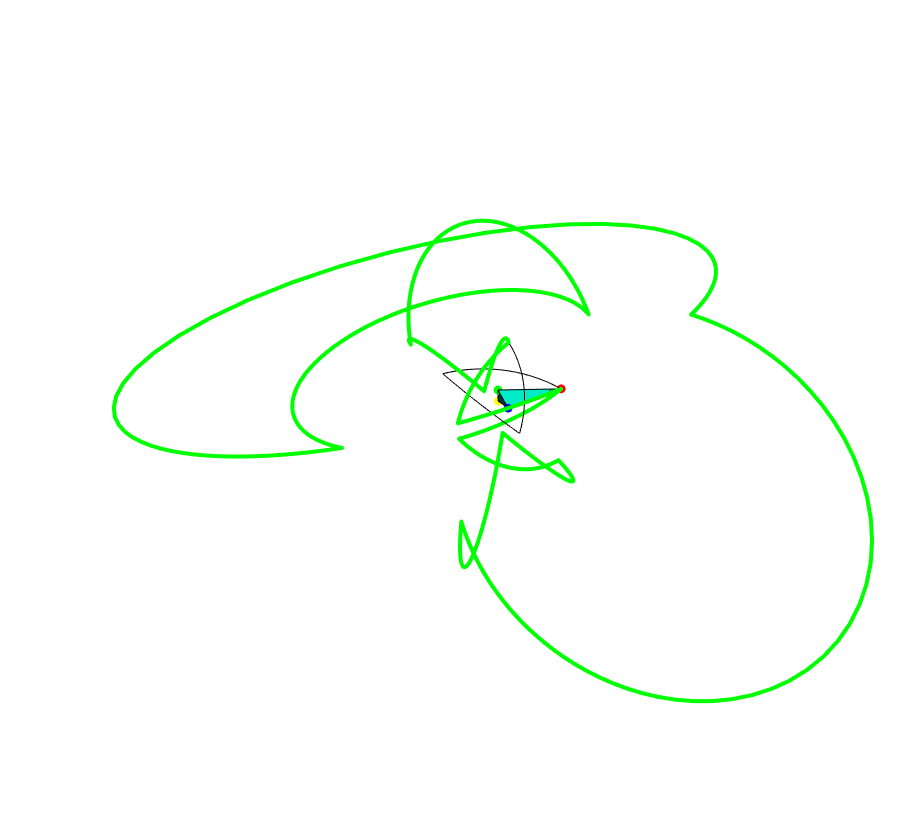
\includegraphics[width=\linewidth]{img2}
		\caption{Stereographic projection of the basic face of $\left\{\frac{12}{1,5},3,5\right\}$}
	\end{figure}
	

\clearpage
\section{Appendix}
\subsection{Further details on $\left\{\frac{12}{1,5},3,5\right\}$}
The intersection property follows by Lema 11 in \cite{schulte-chiral} from
\[\langle S_1\rangle\cap\langle S_2\rangle=\{\Id\}=\langle S_2\rangle\cap\langle S_3\rangle\qquad\text{and}\qquad \langle S_1,S_2\rangle\cap\langle S_2,S_3\rangle=\langle S_2\rangle\]
The following also hold for the resulting polytope on the dual construction:
\begin{enumerate}
	\item $\Stab_{\langle S_1,S_2\rangle}(v)=\langle S_2\rangle$.
	\item $\Stab_{\langle S_1,S_2\rangle}(f)=\langle S_1\rangle$.
	\item $\Stab_{\langle S_1,S_2\rangle}(e)=\langle S_1S_2\rangle$
	\item $\Stab_{\langle S_1,S_2,S_3\rangle}(v)=\langle S_2,S_3\rangle$.
	\item $\Stab_{\langle S_1,S_2,S_3\rangle}(e)=\langle S_1S_2,S_3\rangle$
	\item $\Stab_{\langle S_1,S_2,S_3\rangle}(f)=\langle S_1,S_2S_3\rangle$
	\item $\Stab_{\langle S_1,S_2,S_3\rangle}(c)=\langle S_1,S_2\rangle$
\end{enumerate}
In $\left\{\frac{12}{1,5},3,5\right\}$, there are
\begin{itemize}
	\item 12 vertices and edges in every face
	\item 48 vertices in every cell
	\item 120 vertices in total
	\item 72 edges in every cell
	\item 720 edges in total
	\item 12 faces in every cell
	\item 300 faces in total
	\item 50 cells in total
\end{itemize}

\end{document}